\documentclass[10pt]{article}
\usepackage[margin=0.8in]{geometry}
\usepackage[utf8]{inputenc}
\usepackage[T1]{fontenc}
\usepackage[english]{babel}

\usepackage{fourier}
\usepackage{amsmath}
\usepackage{amssymb}
\usepackage{amsfonts}
\usepackage{amsthm}

\usepackage{graphicx}
\usepackage{float}
\usepackage{caption}
\usepackage{subcaption}
\usepackage{adjustbox} % Good for image handling

\usepackage{booktabs}

\usepackage{etoolbox}
\usepackage{siunitx}
\usepackage{parskip} % Creates space between paragraphs instead of indentation
\setlength{\parskip}{1em} % Adjust space between paragraphs
\setlength{\parindent}{0pt} % No indentation

\usepackage{tikz} % For diagrams
\usetikzlibrary{shapes.geometric, arrows, positioning}

\usepackage{hyperref}
\hypersetup{
    colorlinks=true,
    linkcolor=blue,
    filecolor=magenta,
    urlcolor=cyan,
}
\usepackage{cite}

\usepackage{listings}
\usepackage{color}

\definecolor{codegreen}{rgb}{0,0.6,0}
\definecolor{codegray}{rgb}{0.5,0.5,0.5}
\definecolor{codepurple}{rgb}{0.58,0,0.82}
\definecolor{backcolour}{rgb}{0.95,0.95,0.92}

\lstdefinestyle{mystyle}{
    backgroundcolor=\color{backcolour},
    commentstyle=\color{codegreen},
    keywordstyle=\color{magenta},
    numberstyle=\tiny\color{codegray},
    stringstyle=\color{codepurple},
    basicstyle=\ttfamily\footnotesize,
    breakatwhitespace=false,
    breaklines=true,
    captionpos=b,
    keepspaces=true,
    numbers=left,
    numbersep=5pt,
    showspaces=false,
    showstringspaces=false,
    showtabs=false,
    tabsize=2,
    language=C++
}
\lstset{style=mystyle}

\newcommand{\code}[1]{\texttt{#1}}


\title{Assignment 4: Hybrid MPI + FastFlow MergeSort}
\author{Luca Lombardo \\ SPM Course a.a. 24/25}
\date{}

\begin{document}

\maketitle
\vspace{-1.5em} % Reduce space after title block


The goal of this project was to develop a scalable MergeSort algorithm for a large array of records, combining intra-node parallelism with FastFlow and inter-node parallelism with MPI.
\section{Implementation Strategy}

At the outset, a key design decision was made regarding the \code{Record} data structure. While the assignment specified a fixed-size payload array (\code{char rpayload[RPAYLOAD]}), we opted for a more flexible structure with a dynamically allocated payload (\code{char* payload}). This choice was motivated by the need for a versatile and robust benchmarking framework. Using a dynamic payload allows the record size to be configured at runtime via command-line arguments, which is very useful for systematic performance analysis across various payload sizes without requiring code recompilation for each test. This design choice does not compromise the performance analysis. The memory for each record's payload is allocated once at the beginning of the tests and remains fixed throughout the sorting process. Within the core sorting algorithms, the cost of moving or comparing these records is dominated by the size of the payload. While this approach introduces a single level of pointer indirection compared to a static array, its impact is negligible for a memory-bandwidth-bound streaming algorithm like MergeSort. The use of move semantics ensures that during merge operations, only the pointer and size are transferred, preserving performance characteristics equivalent to those of a fixed-size struct.

\subsection{Single-Node Parallel Design (FastFlow)}
A classic MergeSort naturally decomposes into two distinct phases: an initial, highly parallel sorting of small data chunks, followed by a series of sequential merge passes. Our implementation mirrors this structure, employing dedicated FastFlow farms for each phase to optimize resource utilization.

The first phase, parallel sorting, addresses the initial data partitioning. The array is divided into numerous small, cache-friendly chunks to maximize data locality. The sorting of these independent chunks represents an embarrassingly parallel problem, for which we employed an \code{ff\_farm}. An emitter node decomposes the array into tasks which are distributed to a pool of worker threads. Each worker leverages \code{std::sort} to sort its assigned chunk in-place.

The second phase, iterative merging, progressively combines the sorted chunks. This process is inherently iterative and is implemented with a loop where, at each iteration, a new \code{ff\_farm} executes a single merge pass in parallel. A critical optimization in this stage is the use of a "ping-pong" buffer strategy. By allocating a single auxiliary buffer and swapping pointers between source and destination at the end of each pass, we eliminate the significant overhead of copying data between merge stages. This out-of-place merge technique is standard for maximizing memory throughput. The merge operation itself is optimized through \code{std::make\_move\_iterator}, ensuring that for our \code{Record} structure, only pointers are moved, not the potentially large payloads, thus minimizing data transfer costs on the memory bus.

\subsubsection{Architectural Considerations and Discarded Alternatives}
The assignment suggested exploring FastFlow's building blocks, including \code{ff\_pipeline} and \code{ff\_all2all}. We evaluated these alternatives but ultimately discarded them for sound performance and algorithmic reasons.

The \code{ff\_all2all} pattern is designed for data redistribution, where each worker sends a piece of its local data to every other worker. This communication pattern is fundamental to algorithms like Radix Sort or Sample Sort but is algorithmically incompatible with MergeSort, which relies on merging physically adjacent, sorted segments in a hierarchical, pairwise fashion.

An integrated pipeline architecture, such as \code{feeder -> sort\_stage -> merge\_stage}, also proved suboptimal. Our benchmarks showed significant performance degradation. This is because MergeSort is fundamentally a Bulk-Synchronous Parallel (BSP) algorithm. There is a hard synchronization point after the initial sort phase; the merge phase cannot begin until all chunks are sorted, precluding any opportunity for true, overlapping pipelining. The inter-stage communication and scheduling overhead introduced by the \code{ff\_pipeline} outweighs any potential benefits compared to the lean approach of dedicating all parallel resources to a single, optimized farm for each distinct computational phase.


\subsection{Hybrid Multi-Node Design (MPI + FastFlow)}
To scale the algorithm beyond a single node, we designed a hybrid implementation that combines MPI for inter-node coordination with our optimized FastFlow MergeSort for intra-node computation. The overall process is structured into three distinct phases.

The first phase is a load-balanced data distribution. The root process (rank 0) partitions the global dataset of size $N$ into $P$ contiguous blocks, where $P$ is the MPI world size. To handle cases where $N$ is not perfectly divisible by $P$, we calculate unique per-process element counts and memory displacements. This information is then used with the collective operation \code{MPI\_Scatterv}, which is more general than a simple \code{MPI\_Scatter} and ensures an even distribution of records. For efficiency, especially with non-trivial payloads, data is first serialized into a contiguous byte buffer. This strategy minimizes the number of discrete MPI calls and optimizes for network throughput by sending a single, large message chunk to each process.

The second phase is local sorting. Upon receiving its data partition, each MPI process executes a multi-threaded parallel mergesort. This step performs a coarse-grained, computation-bound sort on the local data, leveraging all available cores on the node as configured. This transforms the global problem into a set of $P$ distributed, independently sorted arrays, preparing the data for the final merge phase.

The third and most complex phase is hierarchical merging. After local sorting, the distributed segments must be merged into a single, globally sorted array at the root. We chose a binary tree reduction pattern for this task, which completes in $\log_2(P)$ communication steps. At each step, active processes are paired: a "sender" transmits its data to a "receiver," which then performs a two-way merge. This pattern effectively distributes the merge workload across multiple nodes in the early stages, but progressively serializes the work toward the root process, which performs the final merge.

A critical aspect of this phase is the communication strategy, designed to maximize computation-to-communication overlap. Our implementation employs a non-blocking model based on \code{MPI\_Isend} and \code{MPI\_Irecv}. This approach decouples the initiation of a data transfer from its completion, allowing the program to continue execution. A receiving process posts a non-blocking receive for an expected data chunk and then enters a progress-checking loop. By repeatedly polling the status of the transfer with \code{MPI\_Test}, the process can begin merging data from a completed transfer immediately, even while other network operations are still in flight. This design aims to hide the communication latency and bandwidth costs of one transfer behind the computational work of a concurrent merge operation, thereby improving overall resource utilization.

\subsubsection{Alternative Merge Strategy: Centralized K-Way Merge}
We also evaluated an alternative strategy for the final merge phase: a centralized k-way merge. In this model, all $P-1$ non-root processes send their locally sorted data directly to the root process, which then performs a single, large k-way merge using a min-heap data structure.

Theoretically, this approach is attractive as it reduces the number of communication rounds from $\log_2(P)$ to one. However, our benchmarks showed it to be less performant than the binary tree reduction. The primary reason is that it creates a massive communication and computation bottleneck at the root process. The root must handle incoming network traffic from all other processes simultaneously while also performing the entire merge. This serializes a large fraction of the work and leaves the other nodes idle after their initial send. In contrast, the binary tree approach distributes the merge workload across multiple nodes in the initial steps, leveraging the computational power of the entire system for a longer duration.

\clearpage
\section{Performance Analysis}
We benchmarked our implementations to evaluate their strong and weak scaling properties. The analysis is based on the data collected and visualized below.

\begin{figure}[H]
    \centering
    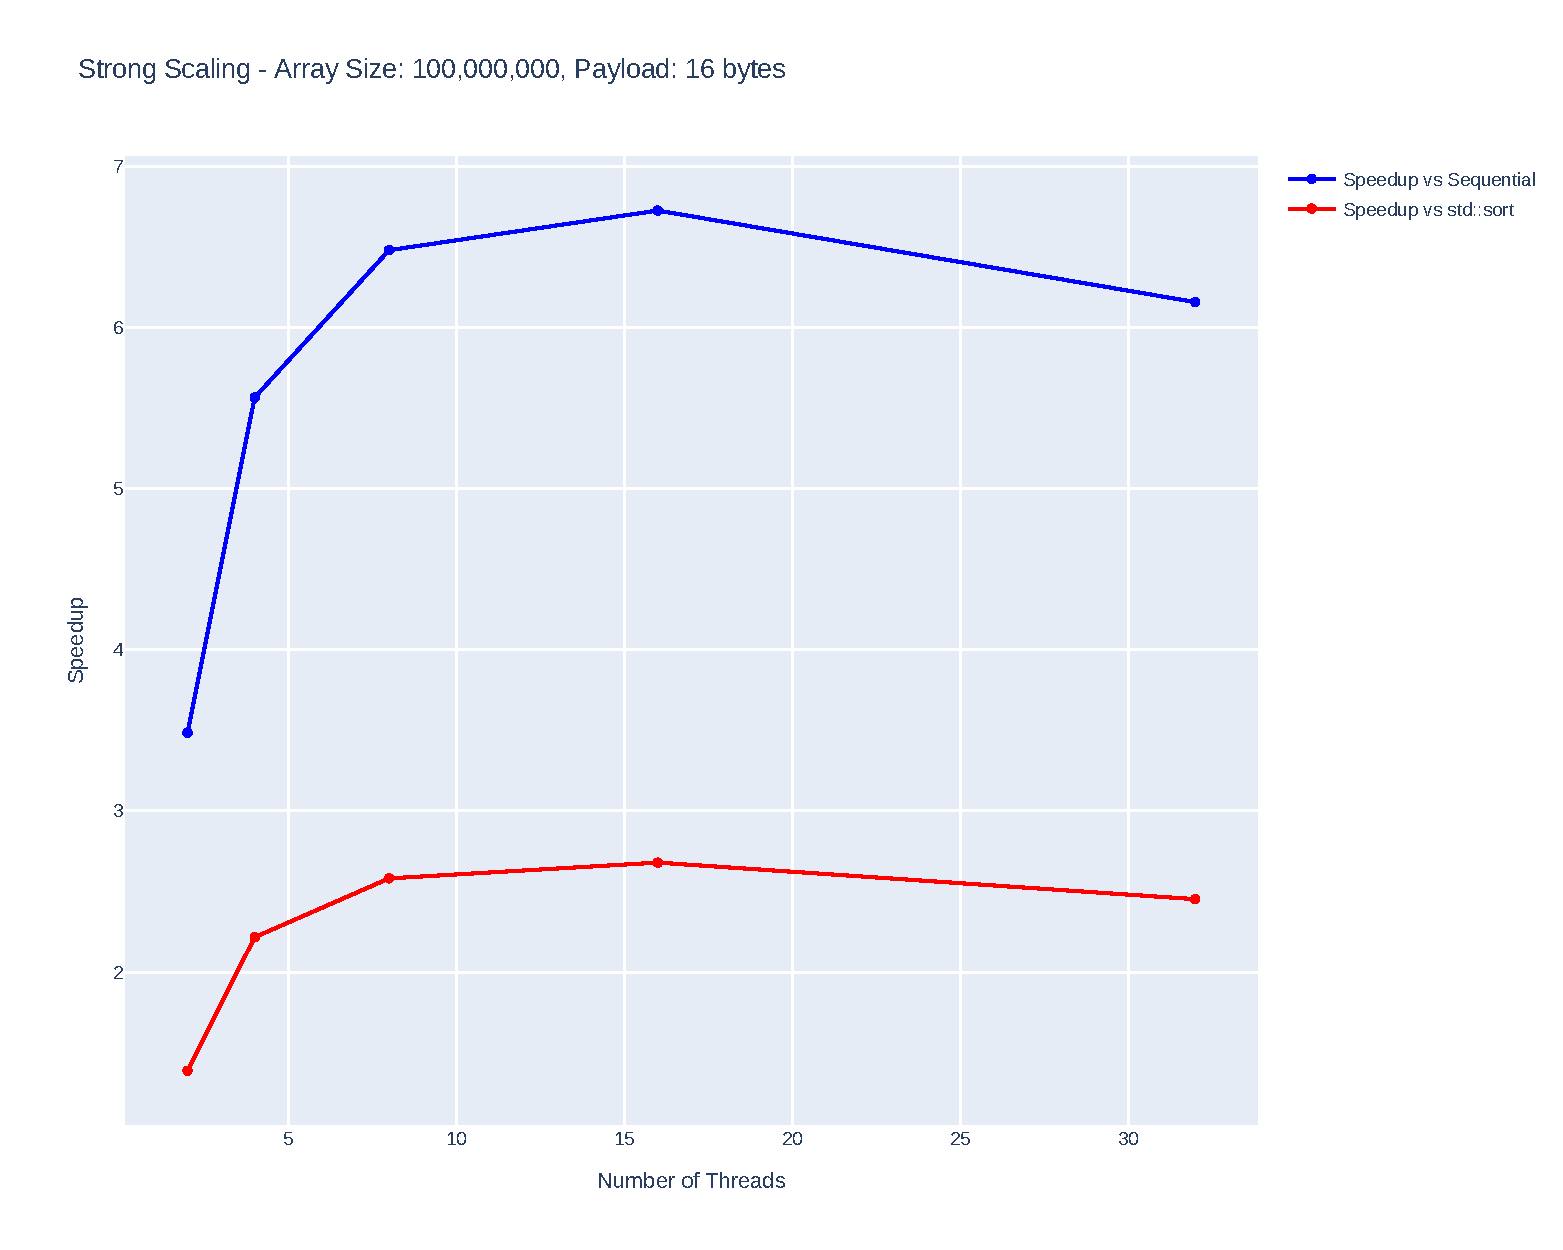
\includegraphics[width=0.6\linewidth]{../python/plots/strong_scaling.pdf}
    \caption{Single-node strong scaling analysis.}
    \label{fig:strong_scaling}
\end{figure}

Figure \ref{fig:strong_scaling} shows the strong scaling of our FastFlow implementation. The speedup increases significantly up to 16 threads, reaching a peak of approximately 6.8x against our sequential implementation. Beyond this point, performance saturates and then begins to degrade. This behavior is an expected illustration of Amdahl's Law, where the parallel overhead, including thread management, synchronization, and memory bus contention, becomes a dominant factor. As the number of threads grows, the marginal gain from additional parallelism diminishes until it is negated by these overheads, defining an optimal level of concurrency for this specific problem size and architecture.

\begin{figure}[H]
    \centering
    \begin{subfigure}{0.49\textwidth}
        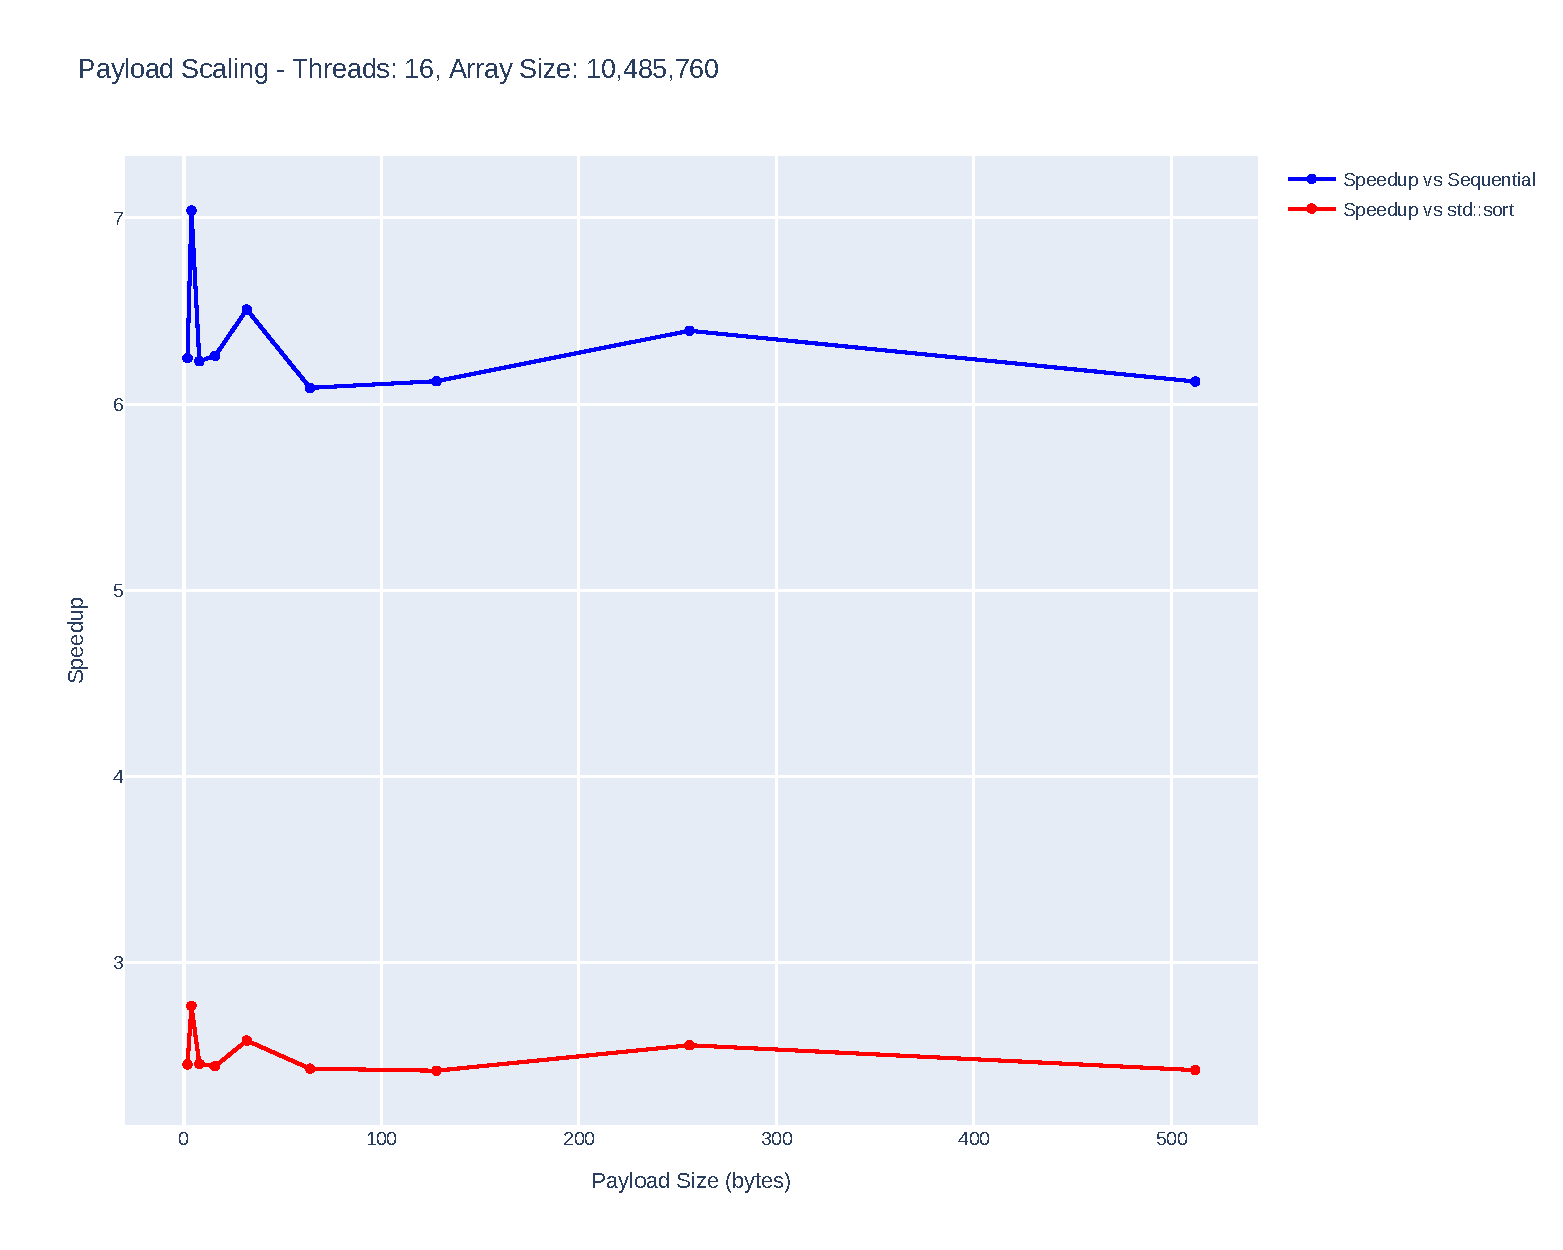
\includegraphics[width=\linewidth]{../python/plots/payload_scaling.pdf}
        \caption{Payload size sensitivity analysis.}
        \label{fig:payload_scaling}
    \end{subfigure}
    \hfill
    \begin{subfigure}{0.49\textwidth}
        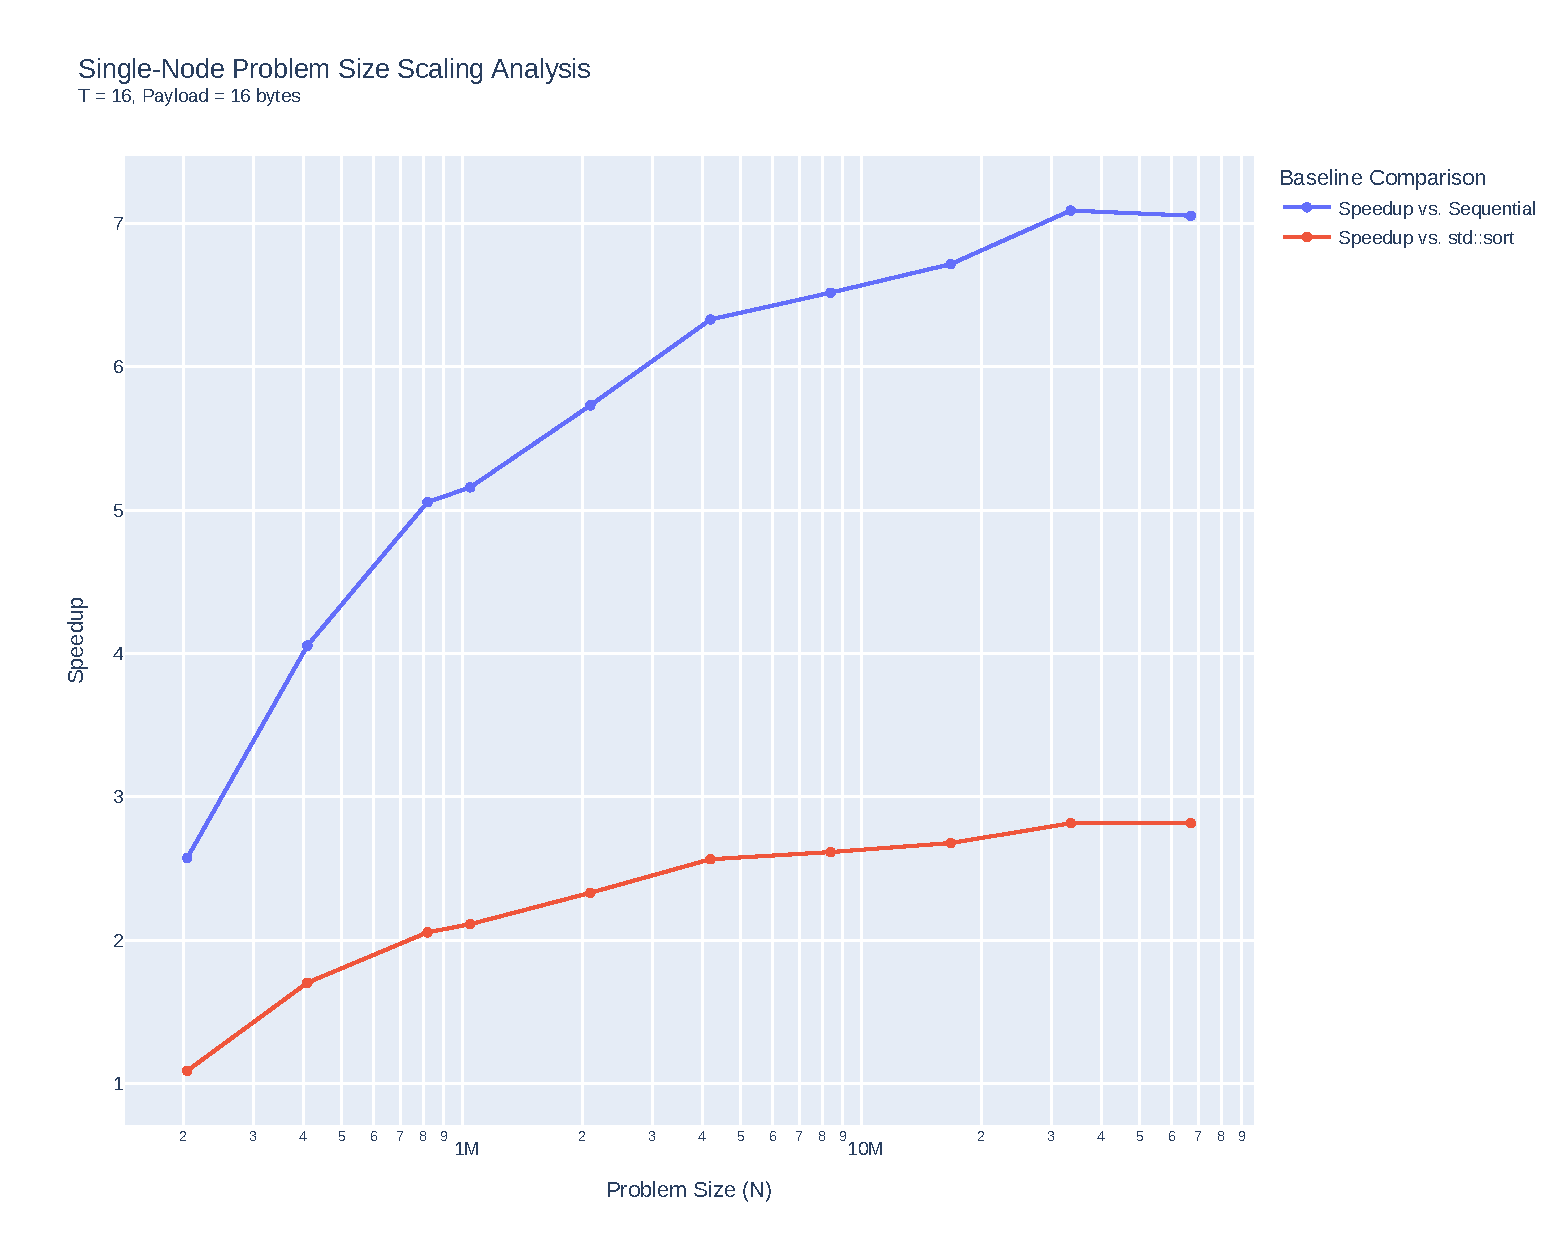
\includegraphics[width=\linewidth]{../python/plots/weak_scaling.pdf} % Note: this is actually Problem Size scaling
        \caption{Single-node problem size scaling.}
        \label{fig:problem_size_scaling}
    \end{subfigure}
    \caption{Single-node performance sensitivity to payload and problem size.}
    \label{fig:single_node_sensitivity}
\end{figure}

The impact of payload size is shown in Figure \ref{fig:payload_scaling}. The execution time remains relatively stable for payloads from 8 to 512 bytes. This indicates that the algorithm's performance is heavily influenced by the system's memory bandwidth. The primary cost in the merge phase is data movement, which scales linearly with the record size. As the payload grows, the problem transitions from being potentially latency-sensitive to firmly memory-bandwidth-bound. The time spent in CPU-bound computation (key comparisons) becomes negligible compared to the time the memory subsystem spends satisfying data transfer requests.

Figure \ref{fig:problem_size_scaling} presents a scaling analysis where the number of threads is fixed, and the total problem size is increased. It is important to note that the x-axis (Problem Size) is plotted on a logarithmic scale. The speedup exhibits strong growth with the problem size, appearing almost linear on this log-scale plot, which indicates a highly favorable scaling behavior. This aligns with the principles of Gustafson's Law: by increasing the problem size, the serial fraction of the work becomes less significant relative to the parallelizable portion. With more data to process, the initial fixed costs of setting up the FastFlow framework and threads are amortized over a longer execution time, leading to substantially better efficiency and speedup.

\begin{figure}[H]
    \centering
    \begin{subfigure}{0.49\textwidth}
        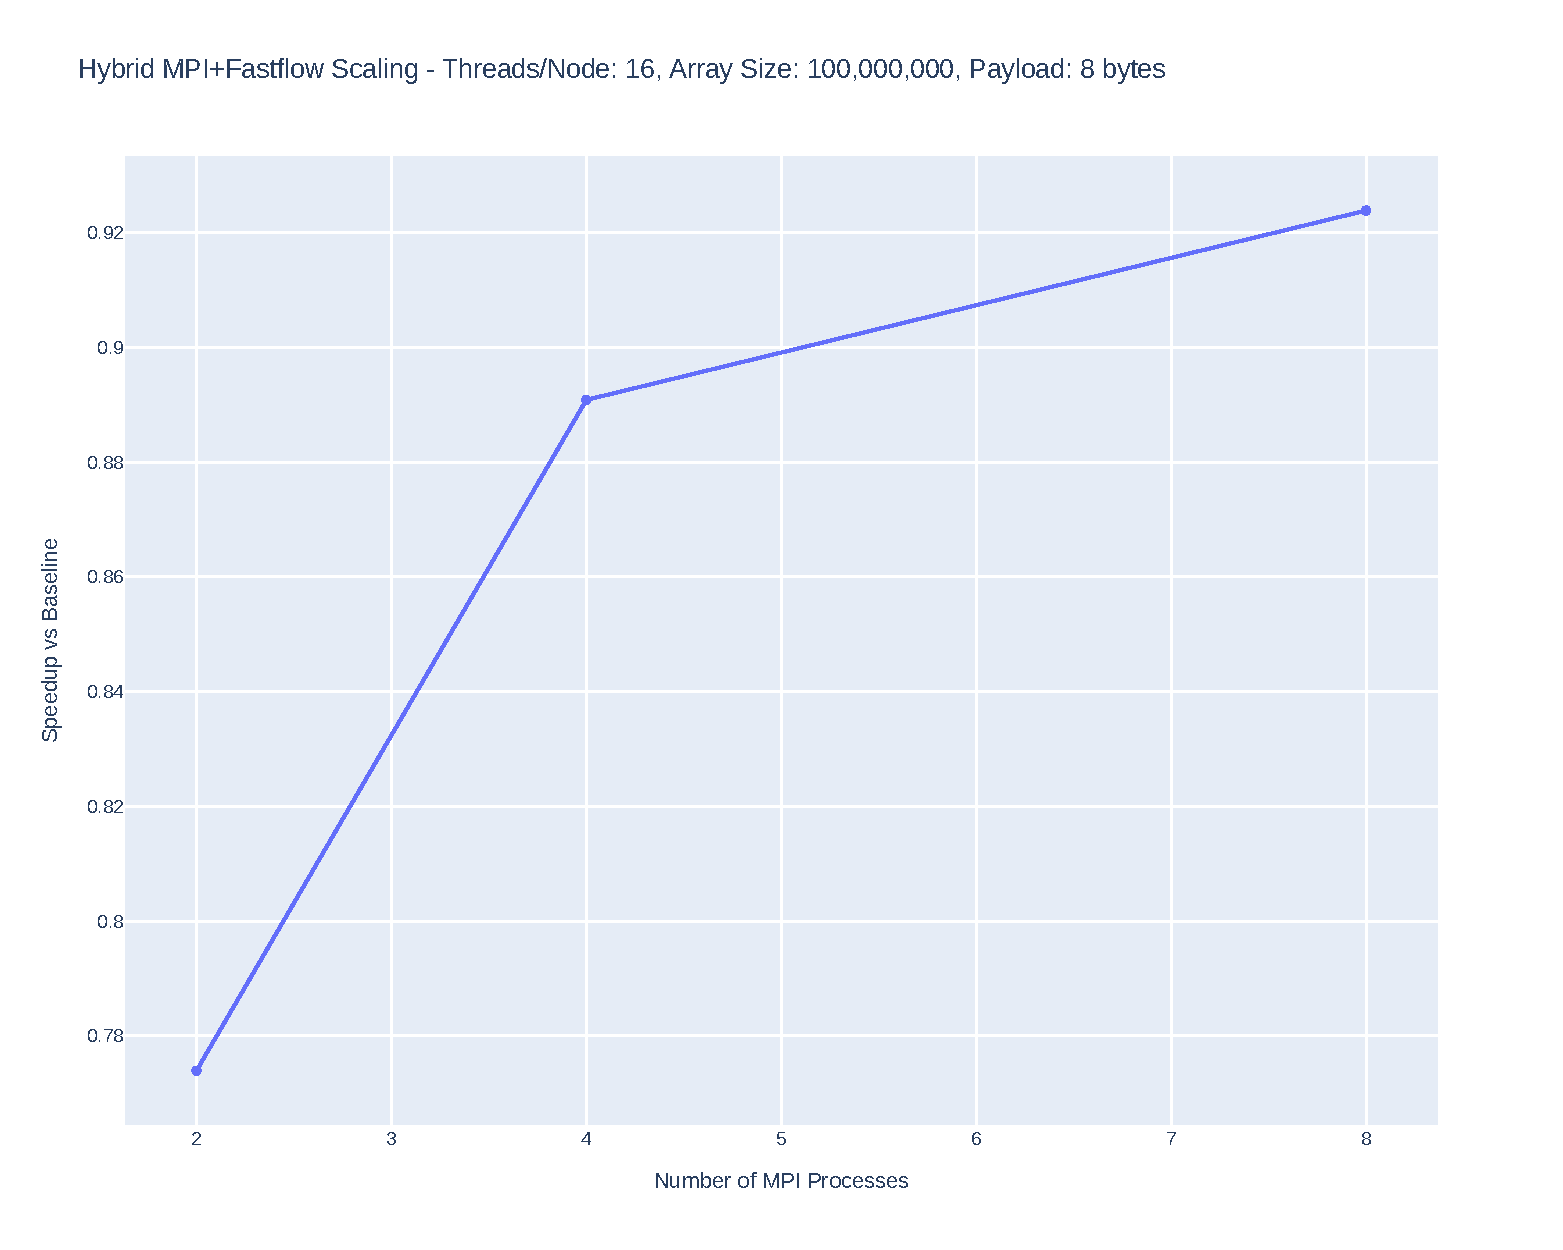
\includegraphics[width=\linewidth]{../python/plots/cluster_scaling.pdf}
        \caption{Cluster strong scaling (MPI).}
        \label{fig:cluster_strong_scaling}
    \end{subfigure}
    \hfill
    \begin{subfigure}{0.49\textwidth}
        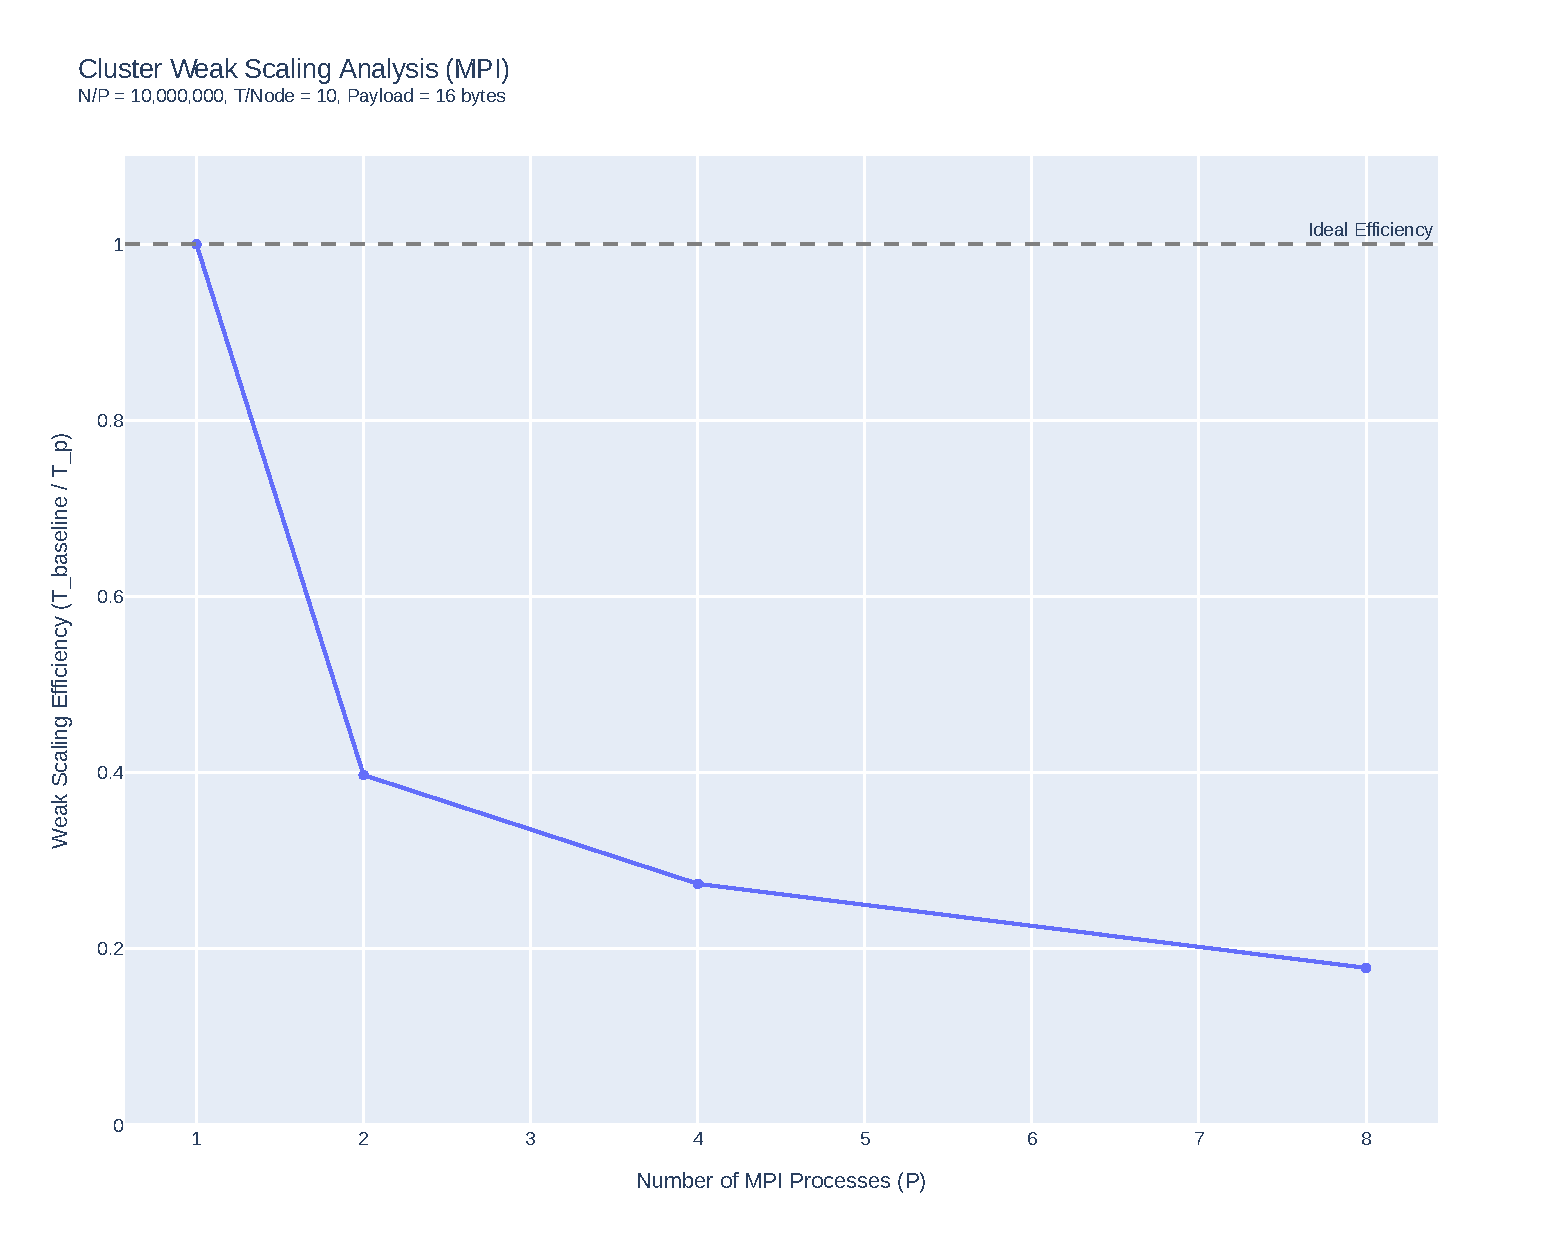
\includegraphics[width=\linewidth]{../python/plots/cluster_weak_scaling.pdf}
        \caption{Cluster weak scaling (MPI).}
        \label{fig:cluster_weak_scaling}
    \end{subfigure}
    \caption{Distributed performance analysis: strong and weak scaling on the cluster.}
    \label{fig:cluster_analysis}
\end{figure}

Figure \ref{fig:cluster_strong_scaling} provides an instructive view into the strong scaling characteristics of the hybrid algorithm. The speedup is measured relative to an optimized single-node parallel baseline, executed via the same framework but constrained to a single MPI process. The results show that for a problem size of 100 million records, the speedup remains sub-linear and below 1.0, indicating that the overhead of distributed execution surpasses the gains from parallel computation across nodes. This outcome stems from the algorithm's communication-to-computation ratio. The total execution time is dominated by two main communication phases: the initial data distribution via \code{MPI\_Scatterv} and, more critically, the iterative binary tree reduction. According to a simple linear cost model, each merge step introduces a latency component ($t_0$) and a bandwidth-dependent term ($n \cdot s$). In our hierarchical merge, the message size ($n$) grows exponentially at each step toward the root. Even with non-blocking primitives like \code{MPI\_Isend} and \code{MPI\_Irecv}, the sheer volume of data being serialized into byte buffers and transferred across the network creates a bandwidth bottleneck that the local computation phases cannot fully hide. The observed performance suggests that for this problem scale, the cumulative communication costs are not sufficiently amortized, leading to a performance penalty compared to the single-node execution.

To complete the performance study, we conducted a weak scaling test on the cluster, where the computational load per node ($N/P$) was held constant. Figure \ref{fig:cluster_weak_scaling} plots the resulting efficiency, which ideally should remain at 1.0. Our results, however, demonstrate a rapid degradation in efficiency. While the local computation phase exhibits perfect weak scaling, the communication complexity of the hierarchical merge phase increases with $P$. Although each process participates in a logarithmic number of steps ($\log_2 P$), the volume of data transferred in the later stages of the reduction grows linearly with the number of nodes participating in a given subtree. This leads to increased network contention and serialization at the upper levels of the merge tree, where fewer processes are active but must handle larger data volumes. Consequently, the total execution time becomes dominated by communication.

\end{document}
